\documentclass[a4paper, 10pt]{article}
\usepackage[left=1in, right=1in, top=1in]{geometry}
\usepackage{listings}
\usepackage{graphics} % for pdf, bitmapped graphics files
\usepackage{graphicx} % for pdf, bitmapped graphics files
\usepackage{color}
\usepackage{cite}
\usepackage{url}
\usepackage{float}

\definecolor{dkgreen}{rgb}{0,0.6,0}
\definecolor{gray}{rgb}{0.5,0.5,0.5}
\definecolor{mauve}{rgb}{0.58,0,0.82}

\lstset{frame=tb,
  language=Bash,
  aboveskip=3mm,
  belowskip=3mm,
  showstringspaces=false,
  columns=flexible,
  basicstyle={\small\ttfamily},
  numbers=none,
  numberstyle=\tiny\color{gray},
  keywordstyle=\color{blue},
  commentstyle=\color{dkgreen},
  stringstyle=\color{mauve},
  breaklines=true,
  breakatwhitespace=true,
  tabsize=3
}
\title{\Large \bf
The impact of leader election strategy on Paxos-based state machine replication
}

\author{Vincenzo Bazzucchi \\ Semester project supervised by Karolos Antoniadis and Dragos-Adrian Seredinschi}%$^{1}$}

\begin{document}

\maketitle
\thispagestyle{empty}
\pagestyle{empty}


\begin{abstract}
State machine replication is a general method for implementing fault-tolerant services. Server replicas rely on a consensus algorithm to agree on the requests and on the order in which these are to be executed. A common approach for implementing replicated state machines is to run multiple consensus instances one after the other which allows for some optimization such as using a leader to reduce the burden of the communication required by the consensus algorithm and batching multiple requests in a single consensus instance. What is the impact of the leader election strategy on the throughput of the system?
\end{abstract}

\section{Introduction}
State machine replication relies on a consensus primitive to ensure that all the server replicas (from now \textit{replicas}) execute \textbf{the same commands in the same order}. Here the \textbf{Paxos} \cite{parttimeLamp}\cite{psimple} consensus algorithm is considered. After a brief introduction to the algorithm and to state machine replication, an optimization to paxos-based state machine replication will be introduced as well as its implementation in a pre-existing software library before investigating the effects of such optimization.

\subsection{Paxos}
Paxos is probably the most well-known consensus algorithm and it is interesting from the perspective of state machine replication as it is a very flexible two-phase algorithm which allows for optimization.
In order to understand the work presented here and the terminology, a brief overview of the algorithm is provided.

In the first phase of the algorithm, each replica broadcasts \texttt{Prepare(n)} messages where \texttt{n} is the proposal number. Upon receiving the prepare message, replicas respond with \texttt{PrepareOK(n', v)}  where \texttt{v} is the value that the replica is proposing and \texttt{n'} is the largest proposal number that the replica has processed until now. When a replica receives a majority of \texttt{PrepareOK}, it considers the first phase concluded. It can proceed and broadcast \texttt{Propose(n, v)} where \texttt{n} is the largest proposal number among those received by \texttt{PrepareOK} and \texttt{v} the associated value.
Upon receiving proposals, replicas respond with \texttt{Accept(n, v)}  where \texttt{n} is the largest proposal number among those received by \texttt{Propose} messages and \texttt{v} is the associated value. When a replica receives a majority of \texttt{Accept}s it verifies whether any of them contains a proposal number greater than the one it proposed. If this is the case, it restarts the entire process, otherwise it considers \texttt{v} as \textbf{decided}.

\subsection{Paxos-based state machine replication}
The Paxos consensus algorithm can be used to implement a replicated state machine algorithm: clients send commands to replicas which use a sequence of consensus instances to choose the order of execution.
Naively using a sequence of consensus instances can be expensive or even fatal to the application as competing \texttt{Prepare} messages can livelock the application.
To reduce the amount of Prepare messages one of the replicas can be chosen to be the \textbf{leader} thus removing the necessity of the first phase of the algorithm: clients send requests to replicas that forward them to the leader. The leader then only needs to send \texttt{Propose} messages and to wait for a majority of \texttt{Accept} responses. This partitions the life of the application into periods that are called \textbf{views}: a new view is installed when the result of the election of a new leader is completed and a new election is only triggered by the failure of the leader.

\section{Motivation}
The leader, like any other replica, might fail at any time and therefore the algorithm needs to react to such an event by electing a replacement. While the concept and usage of a leader is widely discussed in the literature\cite{raft}, the problem of its election is usually briefly solved using a round robin algorithm. To quote \cite{parttimeLamp}: \textit{"This incident led to a debate about the best way to choose a president. [...] Unfortunately, the outcome of this debate is not known; no record exists of the presidential selection protocol that was ultimately used."}

\section{New election algorithm}\label{newalg}
The reasoning behind this work is that the choice of a replacement might have an impact on the throughput of the system. To empirically validate this thesis, an optimal or simply "better" election strategy was implemented and is described here.

Replicas accumulate the outcome of consensus instances in a \textbf{log} in which each entry $i$ is the result of the $i$-th consensus instance. Multiple consensus instances might be executing in parallel and their results might not be ordered: $i < j$ but the result of the instance $j$ is recorded before the result of the instance $i$. In this case, the log can record the results as they arrive. However \textbf{the execution of the commands must respect the order in which they were issued and the execution cannot proceed to entry $j$ if any instance $i<j$ is missing}. This means that the all the clients that sent requests with id $k > i$ are locked.

A natural election strategy consists therefore in choosing the replica with the smallest number of missing entries in its log such that the minimal number of messages will be needed to bring the new leader up to speed.
In order to do so, \texttt{Prepare(n)} becomes \texttt{Prepare([i,\dots,j, m])} where $i,\dots,j$ are the arrays of the IDs of the missing log entries and $m$ is the ID of the next consensus instance. This allows each replica to inform its peers about the state of its log and to choose as new leader the peer with the smallest number of missing log entries. Moreover having the IDs of all the missing entries enables replicas to break ties using by electing the replica which is the most up to date: if two replicas do not have any gap or if they have the same number of gaps in their logs, the replica with the largest value of $m$ will be elected. If all the replicas have the same number of gaps and the same value of $m$, the replica with the smallest ID becomes the new leader. The algorithm needs to be careful about the number of \texttt{Prepare} messages and to avoid re-electing the replica that was suspected if it is still transmitting some messages.\\
\texttt{PrepareOK} can be augmented as well to contain the log entries that its sender can provide the sender of \texttt{Prepare} with.

The recovery process needs to be adapted: if a replica fails and later respawns, it must be informed about the current and past leaders. A simple recovery algorithm can be designed: the respawned replica broadcasts a \texttt{Recovery(x)} message where \texttt{x} is the view in which the replica crashed and it will receive in response \texttt{RecoveryOK(y, [i, \dots, j])} where $i, \dots, j$ are the IDs of the leaders from view $x$ (excluded) up to the current view $y$ included. This information will be sufficient for the recovering replica to start running the Paxos algorithm as it will retrieve the missing entries later in the life of the service.
\begin{figure}[H]
  \centering
  \label{choice}
  \caption{The leader (crowned replica) crashed. The log of $R2$ is much more up to date than the log of $R1$. What is the impact of choosing $R1$ versus $R2$ as next leader? }
  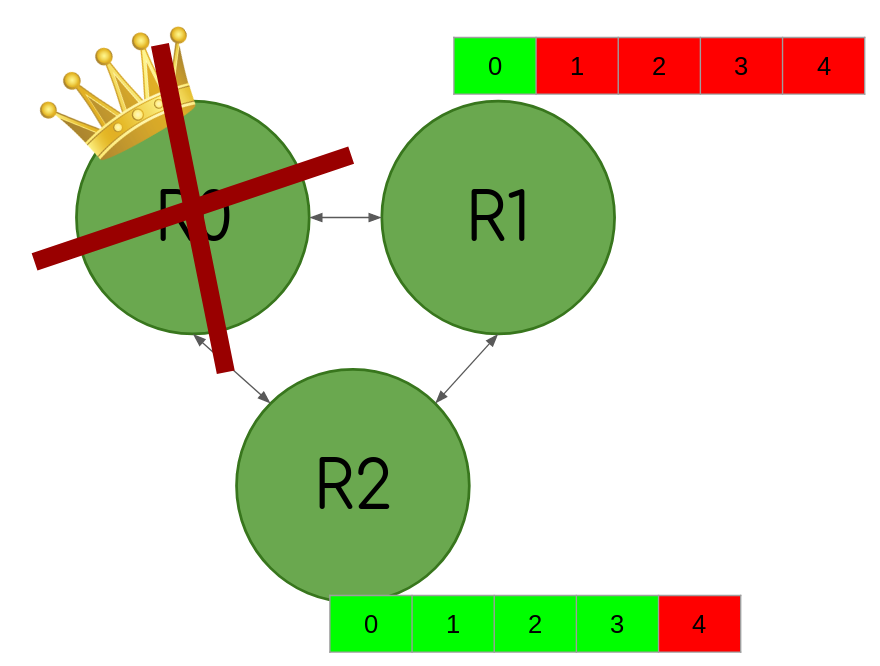
\includegraphics[width=0.5\textwidth]{simplexp.png}
\end{figure}
\section{Implementation}
The algorithm described above was implemented and adapted to the replicated state machine library \textit{JPaxos}\footnote{\url{http://www.it-soa.pl/en/resp/jpaxos/}}. The library is written in the Java programming language and is organized in an object oriented class hierarchy which respects the classical Paxos component division. The library has no external dependencies (beside the SLF4J facilities for application state logging) and provides its users with a simple API to define their own services without having to consider any distributed computing issues except the serialization of the requests and replies used by their application. The library provides some advanced features such as batching of requests and of protocol messages, multiple recovery algorithms and transport protocols.

At the core of the codebase lie the messaging primitives implementing broadcasting and messaging and an \textbf{active failure detector} which relies on timeouts and alive messages to detect whether the current leader failed or is active. The modifications implemented for this project assume that there always exists a \textbf{majority of correct replicas}.
The original implementations relies on the ID of the current view to choose a leader: if we note $v$ the current view (an integer) and $n$ the total number of replicas, the current leader is $v \bmod n$; failure of the leader would result in the increment of $v$ in a scheme similar to round-robin turns.  Most of the implementation of this project consisted in removing the assumption of such an immediate link between the view and the leader identity which was pervasive (and often difficult to locate) across the large codebase.

When the failure detector suspects that the leader crashed, it notifies the Paxos algorithm. At this point the new election algorithm (implemented in the \texttt{paxos.election.LeaderElector} class) can be triggered: the class starts listening and reacts to \texttt{Prepare} messages using the algorithm described above to select the best leader as messages arrive. It considers the election concluded when a majority of \texttt{PrepareOK} messages are received and notifies of its decision the rest of the codebase through some new methods of the storage hierarchy. The storage hierarchy (located in the \texttt{paxos.storage} package) grows in complexity as well: in addition to the log of consensus instances and the current view, the history of leaders and corresponding views must be tracked as well with all the complexity resulting from JPaxos being a multithreaded application where such a history needs to be accessed concurrently by multiple classes on different threads. To evaluate the impact of the election strategy, two classes extend \texttt{LeaderElector}:
\begin{itemize}
    \item \texttt{BestLeaderElector}: implements the algorithm described in section \ref{newalg}
    \item \texttt{WorstLeaderElector}: implements the opposite of the algorithm described in section \ref{newalg}: replicas choose as leader the peer with the largest number of missing log entries 
\end{itemize}

Finally the recovery algorithm needed some alterations. JPaxos used to send \texttt{Recovery} and \texttt{RecoveryOK} messages containing only information about the current view. After receiving a \texttt{RecoveryOK} from the leader, the recovering replica would start the catch up process to retrieve all the entries it had missed during its absence and only after that it would join the Paxos algorithm. Two of the implemented recovery algorithms (\texttt{paxos.recovery.EpochSSRecovery} and \texttt{paxos.recovery.ViewSSRecovery}) were adapted to comply with the separation of leader and view using the algorithm described at the end of section \ref{newalg}. Additionally recovering replicas were prevented from \textbf{triggering the catch up} process after the exchange of recovery messages and to join the Paxos protocol as soon as possible.

\section{Experimental setup}\label{exp}
The setup of an appropriate infrastructure to study the behavior and the throughput of the system was an interesting and challenging exercise as it required collecting
\begin{itemize}
    \item start and completion date of client requests
    \item current leader and election information for each change of view
    \item date and target of \textit{control events} (killing or restarting a replica).
\end{itemize}
Additional complexity arises from the fact that replicas and clients can potentially be deployed on distinct machines, that the data collection must not impact the performances of the algorithm and from the need of \textit{programmatically} controlling the experiments.

The simplest experiment relevant for this work is the following: spawn three replicas, kill one of them (\textbf{not the leader}), accumulate state by keeping the other two active with a stream of requests, restart the killed replica and, as soon as it is running the Paxos algorithm again, kill the leader and observe the behavior of the system. The critical moment in the execution of the simulation is described in figure \ref{choice}: the green entries have been decided and executed while the red ones are still pending. The integers are the identifiers of the consensus instances. The impact on throughput of electing $R1$ versus $R2$ is going to be analyzed.

Here the infrastructure and tools used to conduct and monitor this and other experiments is described.

\subsection{Controlling experiments}
Both clients and replicas need to be started and stopped remotely and programmatically. This requirement was addressed by wrapping the \texttt{Client} and \texttt{Replica} Java classes in new classes \texttt{SpammerClient} and \texttt{ReplicaManager} which expose a HTTP route \texttt{/stop} allowing to kill the corresponding processes. \texttt{SpammerClient} starts issuing requests as soon as it is started while \texttt{ReplicaManager} does not start the Paxos protocol until it receives a request on the \texttt{/start} route. \texttt{ReplicaManager} also responds to \texttt{/status} with information about its leader. Finally in addition to \texttt{/stop} the replica wrapper also exposes \texttt{/kill}: the former is used at the end of the experiment to definitely stop the replica while the former simply kills the replica but keeps listening for \texttt{start} requests.\\
As mentioned in section \ref{exp}, it is necessary to know when the replica is running the Paxos algorithm which might occur some time after it was started. This issue was addressed using \textit{long polling}\footnote{\url{https://en.wikipedia.org/wiki/Push_technology#Long_polling}}: \texttt{ReplicaManager} replies to requests on the \texttt{/start} route only when the Paxos component of JPaxos becomes active, thus special values for the connection timeouts both on the server and client side were necessary.
\begin{figure}[H]
  \centering
  \label{wrappers}
  \caption{The wrappers created to measure the performances of the cluster and to control the experiments}
  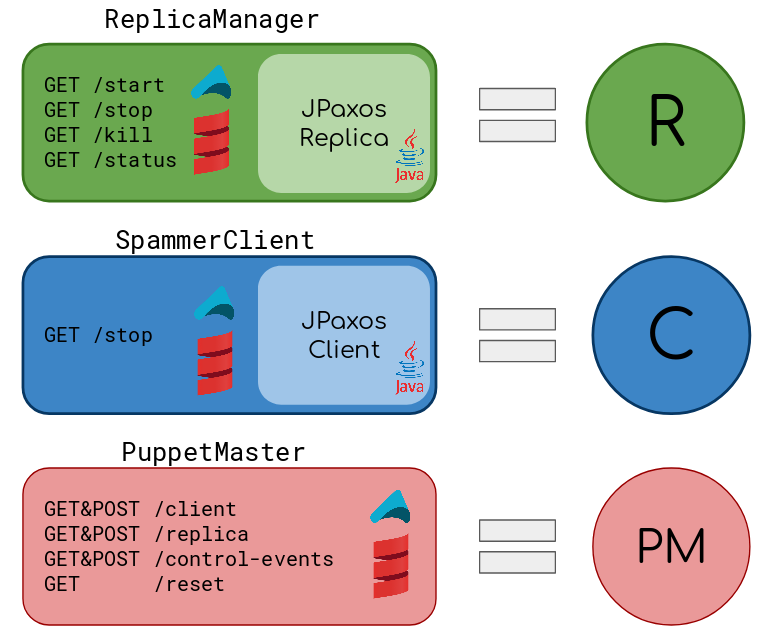
\includegraphics[width=0.6\textwidth]{wrappers.png}
\end{figure}
Both wrappers are written using the Scala programming language\footnote{\url{https://www.scala-lang.org/}} and leveraging the Akka-HTTP library\footnote{\url{https://akka.io/}} and the sbt\footnote{\url{https://www.scala-sbt.org/}} build tool to generate deployable JARs. The experiment itself is then simply defined in a bash script which uses an expressive and simple language based on the primitives \texttt{kill\_replica, start\_replica, run, stop, sleep}. All these functions (except sleep\footnote{\url{https://en.wikipedia.org/wiki/Sleep_(command)}}) are defined in a small bash library (\texttt{experiment.sh}) and are imported at the beginning of the experiment definition. The client-side HTTP implementation used by the bash script is the curl\footnote{\url{https://curl.haxx.se/}} command line tool. An example of experiment definition is given in Listing \ref{simpleexperiment}

\begin{lstlisting}[label=simpleexperiment, caption=Example of experiment definition file]
#!/bin/bash
. ./experiment.sh

replicas=3
clients=1
pmaddress="localhost:9090"

./experiment_cli.sh run $replicas generated-paxos.properties $clients $pmaddress
notifyPM $pmaddress "Experiment started"
sleep 15s

leader="$(get_leader)"
nonleader="$((($leader + 1) % $replicas))"

kill_replica $nonleader
notifyPM $pmaddress "$nonleader killed"
sleep 90s

start_replica $nonleader
notifyPM $pmaddress "$nonleader recovered"

kill_replica $leader
notifyPM $pmaddress "$leader killed"
sleep 10s

notifyPM $pmaddress "End of experiment"
./experiment_cli.sh stop $replicas $clients
\end{lstlisting}

\subsection{Collecting statistics}
The metric considered for this work is the throughput of the system observed by the clients. To measure its value, a very simple register service was implemented: a single integer variable with only two possible commands: read and write. \texttt{SpammerClient} relies on Java's random number generator and on Akka streams to create an infinite stream of commands. The client then processes the elements of the stream one at a time recording the date when it issues the command and when it receives the response and wraps both values (long integers) together with its unique ID in a message that is appended to an asynchronous stream which is mapped to a stream of HTTP requests directed to a microservice called \texttt{PuppetMaster}. Akka is used to implement this asynchronous stream which is treated independently from the rest of the Paxos protocol to avoid slowing it down with expensive operations such as JSON serialization and the TCP/HTTP protocols.

\texttt{ReplicaManager} streams some logging events to \texttt{PuppetMaster} using the same structure: each change of view, the corresponding election result and the date of the event are serialized into a JSON payload and transmitted to study the behavior of the program.

Finally the bash functions defining the experiment transmit the date and label of the "control events" (killing a replica, starting a replica, start/stop of the experiment) to \texttt{PuppetMaster}.

\texttt{PuppetMaster} is implemented in Scala using the Akka framework.

 \begin{figure}[H]
  \centering
  \label{setup}
  \caption{The entities involved in the experiments and their connections}
  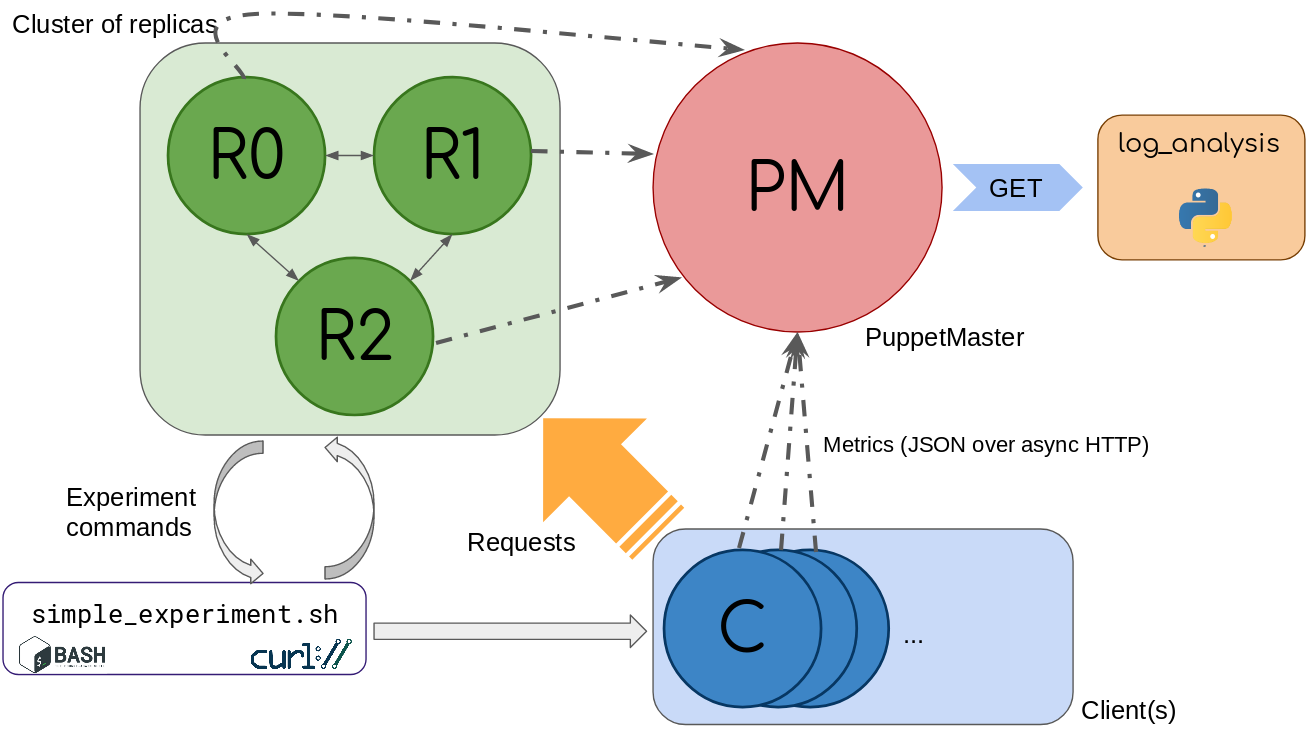
\includegraphics[width=\textwidth]{infrastructure.png}
\end{figure}

\subsection{Statistics analysis}
At the end of the experiment the history of the events can be requested to \texttt{PuppetMaster} through dedicated HTTP routes. Fetching and building an intermediate version of the experiment data is implemented in the \texttt{Experiment} class which also provides some facilities to be serialized into the pickle\footnote{\url{https://docs.python.org/3/library/pickle.html}} binary file format. This allows to programmatically execute multiple experiments one after another, to fetch the corresponding data, compute statistics and serialize everything into files for later analysis. Finally the \texttt{Experiment} class implements a method for plotting the throughput of the system during the experiment along with the control events.

In particular, \texttt{Experiment} is responsible for computing the throughput based on the events logged by \texttt{SpammerClient}: it allocates an array with one entry for each unit of time (i.e. a second) before iterating over the timings sent by each \texttt{SpammerClient}. For each of these events there are two possibilities:
\begin{itemize}
    \item The event starts and completes in the same time window (i.e. in the same second). In this case the throughput for the time window can be increased by 1.
    \item The event starts and completes in different time windows. In this case the to each time window is added the fraction of the event that occurs in that time window.
\end{itemize}

The log analysis code is implemented in the Python prorgramming language\footnote{\url{https://www.python.org/}} using the numpy\footnote{\url{http://www.numpy.org/}}, matplotlib\footnote{\url{https://matplotlib.org/}} and requests\footnote{\url{http://docs.python-requests.org/en/master/}} libraries.

\section{Results}
The experiment described in section 5 was run multiple times varying the number of clients. The experiment code uses the same parameter as the one reported in Listing \ref{simpleexperiment} and modifies the \texttt{clients} variable, accumulating state for $90$ seconds after killing the non-leader replica.
For each value of the number of clients, both \texttt{BestLeaderElector} and \texttt{WorstLeaderElector} were evaluated $5$ times and the execution with the \textit{best performance} was retained for \texttt{BestLeaderElector} while the \textit{worst performance} was retained for \texttt{WorstLeaderElector}.
Comparing the best case of \texttt{BestLeaderElector} to the worst case of \texttt{WorstLeaderElector} provides an intuitive upper bound on the possible benefit of adopting an improved leader election strategy.\\
The discriminant performance statistic is the \textbf{total amount of client commands satisfied after killing the leader}. The results are reported in the following table:

\begin{center}
\begin{tabular}{c|c|c|c}\label{totals}
    Number of clients & \texttt{Best} & \texttt{Worst} & Ratio \texttt{Best}$/$\texttt{Worst} \\ \hline
    2 & $599.16$ & $583.2$ & $1.03$    \\
    4 & $2851.55$ & $1151.94$ & $2.48$ \\
    6 & $470793$ & $4031.69$ & $1.17$  \\
    8 & $6470.26$ & $5555.92$ & $1.17$
\end{tabular}
\end{center}
The table shows that a slightly optimized algorithm for leader election can have a significant impact on the worst case performances of the service.
The impact of the election strategy is also visible in the plots showing the throughput during the experiment in figure \ref{plots}: the worst leader elector causes an interval of 0 throughput longer that the one measured when using the the improved leader elector.

\begin{figure}[H]
    \label{plots}
    \caption{Impact of the leader election strategy on a 3-replicas cluster with different number of clients}
    \centering
    \begin{tabular}{c}
        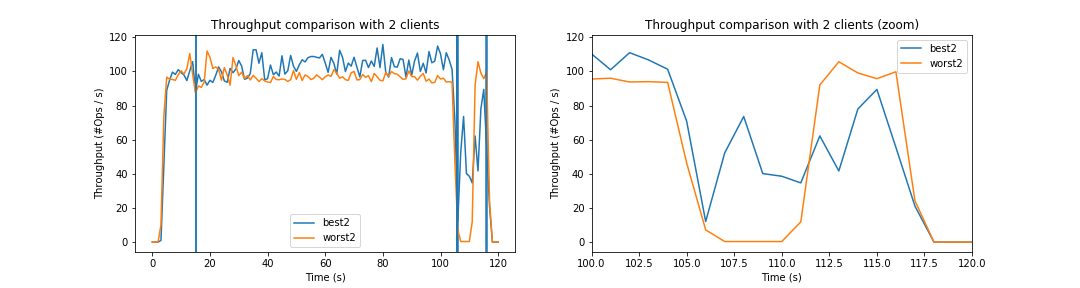
\includegraphics[width=\textwidth]{comp2} \\
        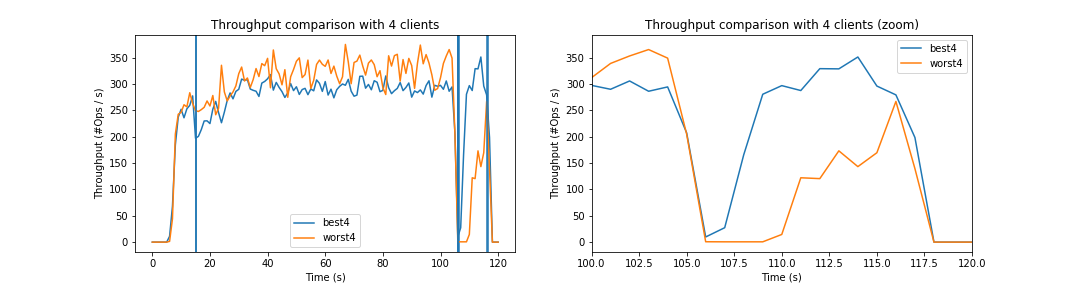
\includegraphics[width=\textwidth]{comp4} \\
        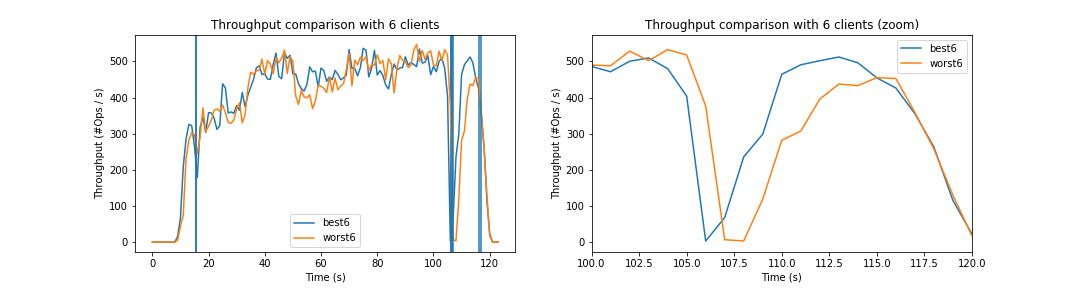
\includegraphics[width=\textwidth]{comp6} \\
        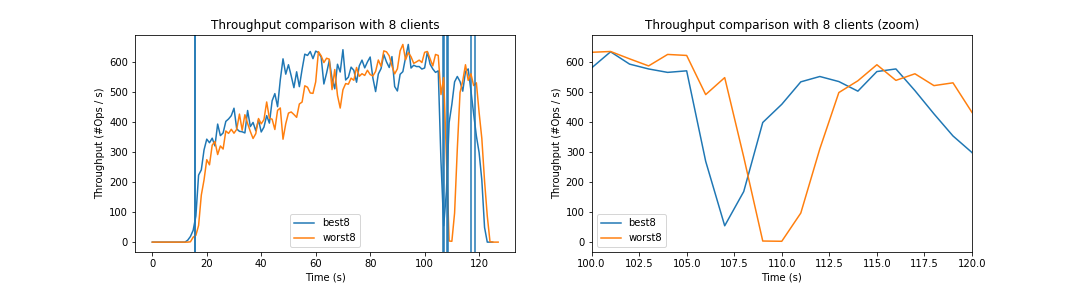
\includegraphics[width=\textwidth]{comp8} \\
    \end{tabular}
    \label{experiment}
\end{figure}

\section{Conclusion}
The results presented above are limited due to the lack of documentation of the JPaxos library which hid the fact that some configurations of parameters are not valid but are accepted by the program and cause unexpected behavior and crashes during the life of the applications. Finding and solving these issues took a lot of time and was quite difficult.

More experiments are thus needed to evaluate the impact of the improved election strategy not only in worst case scenarios but also on average to assess whether modifying current implementations of replicated state machines is worth the complexity and difficulties inherent to developing distributed systems. This project provides a general framework for conducting such experiments on a single machines or on multiple nodes and to collect and analyze the results. Additionally the encouraging results suggest that a small additional complexity in the algorithm could potentially have important repercussions on the overall performance.

\bibliography{refs}{}
\bibliographystyle{plain}

\end{document}
